%%%%%%%%%%%%%%%%%%%%%%%%%%%%%%%%%%%%%%%%%%%%%%%%%%%%%%%%%%%%%%%%%%%%%%%%%%%%%
\chapter{Entwicklung und Umsetzung des Prototyps}
\label{chap:intro}
%%%%%%%%%%%%%%%%%%%%%%%%%%%%%%%%%%%%%%%%%%%%%%%%%%%%%%%%%%%%%%%%%%%%%%%%%%%%%
\chapterstart

Um die Unterschiede bezogen auf Latenz und Performance von REST, GraphQl, gRPC und gRPC-Web in einem konkreten Anwendungsfall zu ermitteln, wurde ein Prototyp entwickelt, mithilfe dessen Messungen zwischen einer Frontend- und Backendanwendung durchgeführt werden können. 
Bei den Messungen wurde die Zeit des Datenaustauschs zwischen den zwei Kommunikationspartnern (End-to-End Latenz) erfasst und anschließend verglichen und analysiert.
Die so gewonnenen Daten sollen anschließend die Basis dafür bilden, 
um die zuvor theoretisch untersuchten Eigenschaften der Technologien unter realen Bedingungen zu überprüfen.

\begin{figure}[htbp]
	\centering
	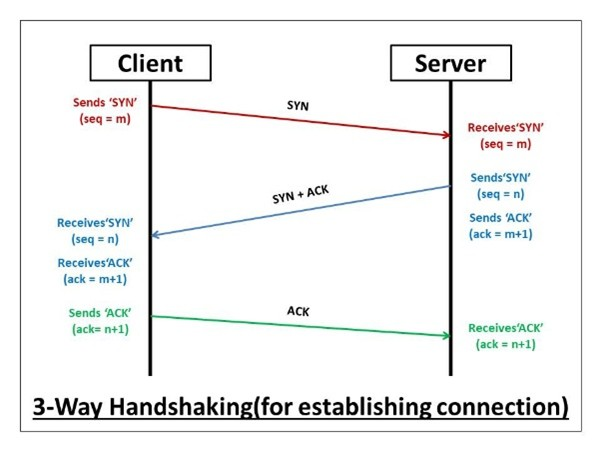
\includegraphics[width=0.7\textwidth]{images/http1_theory.jpg}
	\caption{3-Way Handshake (for establishing TCP connection)}
	\label{fig:threewayhandshake}
\end{figure}

\subsection*{Zielsetzung}
Ziel des praktischen Teils ist es die Leistungsfähigkeit von den genannten API-Technologien zu untersuchen und gegenüberzustellen. Der Prototyp soll so implementiert werden, sodass für jede Technologie eine vergleichbare Umgebung mit den ähnlichen Bedingungen entsteht. 
Im Fokus der Messungen steht die End-To-End Latenz, also jene Zeitspanne vom Absenden einer Anfrage bis zur vollständigen Verarbeitung und Bereitstellung der Antwort im Client. 

Ziel der Messungen ist es Unterschiede zwischen den Technologien sichtbar zu machen und mit den im Theorieteil ermittelten Daten zu vergleichen.
Auf dieser Grundlage und mit Rücksichtnahme auf den Rechercheteil, werden anschließend Rückschlüsse auf die Eignung der einzelnen Technologie für die Kommunikation zwischen Frontend- und Backend-Anwendungen gezogen.


\section{Versuchsaufbau}
Der entwickelte Prototyp besteht grundsätzlich aus 3 verschiedenen Komponenten: 
Ein Backend-Service, ein Web-Client und ein Microservice ähnlicher Konsolen-Client.

Abbildung X [TO-DO] zeigt den schematischen Aufbau des Versuches.

Die zwei verschiedenen Client-Typen können hierbei mit dem gemeinsamen Backend-System kommunizieren.

Der Schwerpunkt der Messungen liegt in folgenden Bereichen:

\begin{itemize}
	\item Vergleich einzelner und mehrfacher Requests
	\item Einfluss verschiedener Browser
	\item Unterschiede zwischen Microservice-Client und Browser-Client
\end{itemize}

\subsection*{Systemarchitektur:}

\subsubsection*{Front-End Clients:}
Der Versuchsaufbau beinhaltet zwei unabhängige Clients, welche jeweils auf einer unterschiedliche Art auf den Backend-Service zugreifen:
\begin{enumerate}
	\item Web-Client: die Übertragung findet dabei zwischen einem Browser und dem Back-End Service statt. Der Web-Client kann auf die REST, GraphQL und gRPC-Web API zugreifen.
	\item Konsolen Client: die Übertragung findet zwischen einer Micro-Service ähnlichen Konsolenanwendung und dem Back-End Service statt. Der Konsolen Client kann auf die REST, GraphQl, gRPC und gRPC-Web API zugreifen.
	
\end{enumerate}

\subsubsection*{Backend Service:}
Der Backend-Service stellt verschiedene Services zur Verfügung und kann von beiden Front-End Clients Anfragen entgegen nehmen.
Die verschiedenen Services wurden so ausgewählt, sodass die gesendeten Daten möglichst realitätsnahe Anwendungsfälle der Frontend-Backend Kommunikation abdecken.

Grundsätzlich, kann auf 3 verschiedene Services zugegriffen werden:

\begin{itemize}
	\item Text – Service: 
	Der Text-Service stellt einen Text im Datentyp „string“ zur Verfügung. Dabei können mit den Datengrößen 1 kB, 10 kB und 100 kB abgefragt werden.
	
	\item Media – Service:
	Der Media-Service stellt Medien zur Verfügung, die mittels eines byte[] verschickt werden. Bei den Medien handelt sich um ein Bild (4 MB), einer Audio-Datei ( 30 MB) und einer Video Datei ( 100 MB ). 
	
	\item Blog - Service: 
	Bei dem Blog Service handelt sich um einen 10 kB großen Datentypen, der verschachtelt andere Datentypen ( Text - "string", Zahlen - "int" und Datum - "DateTime" ) versendet.
	
\end{itemize}

Die in den Services verwendeten Datentypen, sind die gängigsten Datentypen in der Frontend-Backend Kommunikation.

Alle Services wurden seperat mit den Technologien REST, GraphQl, gRPC und gRPC-Web implementiert und können somit von den jeweiligen Clients abgefragt und verglichen werden.

Abbildung X [TO-DO] zeigt den schematischen Aufbau der Backend-Services.

\subsection*{Testfälle:}
Zur Analyse der Client-Server Kommunikation wurden folgende Testfälle definiert, welche relevante Aspekte der Front-End Kommunikation abdecken und für einen adäquaten Vergleich der API-Technologien herangezogen werden können: 
\begin{itemize}
	\item \textbf{Einzelabfragen - Web-Client (1 Request):} Vergleich der Technologien bei beim senden eines einzelnen Requests. Dies wird jeweils bei jedem der definierten Services und für jede vorhandene Datengröße durchgeführt. Die Abfragen werden jeweils mit REST, GraphQl und gRPC-Web durchgeführt. Die Messungen zeigen Ergebnisse über Latenz und Performance.
	\item \textbf{Mehrfachabfragen - Web-Client ( 20 Requests ):} Analog zum Einzelrequest, wird der Versuch erneut mit Mehrfachabfragen durchgeführt, um zu sehen, wie gut die Technologie skalieren, Ressourcen nutzen und mehrere Requests effizient handhaben kann.  
	\item \textbf{Unterschiede bei der Nutzung von verschiedenen Browsern):} um den Einfluss des Webbrowsers auf die Messungen des Web-Clients zu identifizieren, werden erneut Einzelrequests in verschiedenen Webbrowsern durchgeführt. Durch den Versuch wird festgestellt, ob eine Abhängigkeit des Browsers auf die Technnologie besteht.
	\item \textbf{Einzelabfragen - Konsolen-Client (1 Request):} Analog zu den Einzelrequests des Web-Clients wird der Versuch erneut mit einem mircoservice ähnlichem Konsolenclient durchgeführt. Hierbei wird jedoch auch abgesehen von REST, GraphQl und gRPC-Web die Latenz von gRPC gemessen. Durch den Versuch ist eine Gegenüberstellung der Response Zeiten zwischen den beiden Clients möglich.
\end{itemize}

Da es in Web Browsern nicht möglich ist raw gRPC zu verwenden, konnte diese Messung im Rahmen des Browser-Client-Versuchsaufbaus nicht durchgeführt werden. Um Messwerte zwischen gRPC und gRPC-Web zu vergleichen, und um zu sehen in wiefern sich die Performance zwischen Browser – Backend und Microservice – Backend wurde der zweiter Versuchsaufbau mittels eines Konsolen Clients durchgeführt.

\subsection*{Rahmenbedingungen}
Um einen fairen Vergleich herzustellen, wurden alle Requests ausschließlich mit dem HTTP/2.0 Protokoll durchgeführt und verschlüsselt mit https versendet. Bei der Response-Zeit handelt es sich jeweils um die End-to-End-Latenz aus der Sicht des Nutzers. Es wird dabei die Zeit ab dem Absenden des Requestes bis zu dem Zeitpunkt, ab dem die Daten tatächlichen im Client fertig verarbeitet bereitstehen gemessen. Die Response Zeit beinhaltet also: 

\begin{enumerate}
	\item die Transportzeit über das Netzwerk:
	Zeit für den Hin- und Rückweg des Pakets durch das Netzwerk.
	
	\item Back-End-Verarbeitung:
	Die Serverseitige Bearbeitung des Requests
	
	\item Antwortübertragung:
	Zeit für das Senden der Antwort( inklusive Header und Payload) zurück an den Client.
	
	\item Clientseitige Verarbeitung:
	die Verarbeitung des Responses, sodass die Daten tatsächlich im Client verwendet werden können. (JSON Parsing, Binär-Parser).
	
\end{enumerate}

\clearpage
\section{Implementierung:}
Der Prototyp beinhaltet einen Backendservice, einen Web-Client und einen Konsolen Client. Dieser Abschnitt befasst sich mit der Implementierung der jeweiligen Komponenten. 

Um die Vergleichbarkeit der jeweiligen API-Technologien zu erhöhen, wurden alle Clients und Services so minimalistisch wie möglich umgesetzt, da weitere Frameworks oder Logik die Datenverarbeitung beeinflussen, und somit die tatsächlichen Zeiten verzerren könnten.
Jeder Service liefert ausschließlich den für den Testfall angeforderten Daten. 

Ziel dieses Abschnittes ist es die Architekturentscheidungen, Funktionsweisen sowie die technischen Aspekte darzustellen, auf Basis anschließend die Messungen durchgeführt werden.

\subsection{Backend Service:}

Der Backend Service wurde modular und technisch getrennt umgesetzt, um die Technologien jeweils unabhängig voneinander vergleichen zu können. Die Implementierung basiert auf .NET 9, einer plattformunabhängigen Open-Source-Laufzeitumgebung von Microsoft, die für moderne Web- und Microservice-Anwendungen konzipiert ist.
Die Services stellen für jede der APIs dieselben Daten zur Verfügung und können folgendermaßen Abgefragt werden:

\begin{itemize}
	\item REST: per HTTP-GET auf definierte Endpunkte
	\item GraphQl: über einen einzigen Endpunkt, wobei der Client die benötigten Felder in der Query spezifiziert.
	\item gRPC und gRPC-Web: als typisierte RPC call (HTTP/2, Protobuf) 
\end{itemize}

\begin{figure}[htbp]
	\centering
	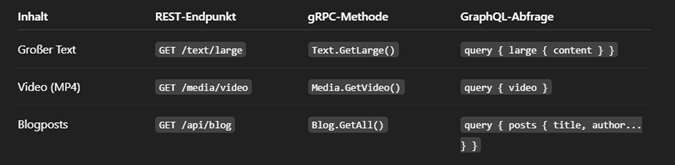
\includegraphics[width=0.7\textwidth]{images/prakt1.png}
	\caption{Daten}
\end{figure}


Die Struktur des Backend-Services gliedert sich in 4 eigenständige Projekte:

\begin{enumerate}
	\item Common:
	Das Common Projekt stellt die Testdaten zentral zur Verfügung. Damit die Testdaten bei einem Request nicht zuerst aus der Datei gelesen werden müssen, werden diese bei Programmstart einmal in den Arbeitsspeicher geladen. Zu diesem Zweck wurde ein API – Cache erstellt, der alle Text und Medienobjekte vorab einliest, die Daten können dann zur Laufzeit direkt vom Cache abgefragt werden.
	
	Für die Testdaten wurden Datentypen die typischerweise an Web Clients gesendet werden ausgwählt und beinhalten:
	
	
	\begin{itemize}
		\item Texte in drei Größen: 1\,kB, 10\,kB, 100\,kB
		\item Medieninhalte: 3\,MB Foto, 30\,MB Audio-Datei, 100\,MB Video-Datei
		\item Strukturierte Binärdaten: ein selbst definierter Datentyp mit verschachtelten Abschnitten, Metadaten, Zahlenblöcken und Autoreninformationen
	\end{itemize}
	\item RestAPI:
	Die REST API wurde mittels einem Controller Muster von ASP.NET Core implementiert und stellt 3 eigenständige Endpunkte zur Verfügung. Die Kommunikation erfolgt ausschließlich über http GET.
	
	Die Controller sind wie folgt definiert:
	
	\begin{itemize}
		\item \textbf{TextController}: Stellt Textdaten in drei Größen zur Verfügung.\\
		\emph{Rückgabeformat}: \texttt{application/json}
		\item \textbf{MediaController}: Stellt ein Bild, eine Audiodatei und ein Video bereit.\\
		\emph{Rückgabeformat}: Binärdaten (\texttt{byte[]}) mit MIME-Type \texttt{image/jpeg}, \texttt{audio/wav}, \texttt{video/mp4}
		\item \textbf{BlogController}: Stellt einen vordefinierten Blogeintrag bereit.\\
		\emph{Rückgabeformat}: \texttt{application/json}
	\end{itemize}
	
	\item GraphQlAPI:
	Die GraphQL-API wurde mittels des \texttt{.NET}-Frameworks \texttt{HotChocolate} implementiert.
	Als Einstiegspunkt wurde eine \texttt{Query}-Klasse definiert, welche für die verschiedenen Services (Text, Medien, Blog) mit jeweiligen Teildateien erweitert wurde.
	
	Folgende Queries wurden definiert:
	\begin{itemize}
		\item \textbf{TextQuery}: Stellt die Felder \texttt{small}, \texttt{medium} und \texttt{large} bereit, welche jeweils Textinhalte als \texttt{string} zurückgeben.
		\item \textbf{MediaQuery}: Stellt die Felder \texttt{image}, \texttt{audio} und \texttt{video} bereit, welche in der GraphQL-Antwort Base64-kodiert übertragen werden.
		\item \textbf{BlogQuery}: Stellt das Feld \texttt{posts} zur Verfügung, welches die für den Blogpost definierten Daten enthält.
	\end{itemize}
	
	Alle Abfragen erfolgen über \texttt{HTTP~POST}-Anfragen an den Endpunkt \texttt{/graphql} und haben das Format \texttt{application/json}.
	
	\item GrpcWebAPI: 
	Die gRPC-Web-API basiert auf den definierten \texttt{.proto}-Dateien (\texttt{text.proto}, \texttt{media.proto}, \texttt{blog.proto}). In den Proto-Dateien wurden sowohl die \emph{Messages} und Datentypen der Testdaten als auch die \emph{Services}, mit denen auf die Messages zugegriffen werden kann, definiert. 
	
	Die Services implementieren folgende Methoden:
	\begin{itemize}
		\item \textbf{TextService}: Rückgabe der drei Textgrößen über die Methoden \texttt{GetSmall()}, \texttt{GetMedium()} und \texttt{GetLarge()}.\\
		\emph{Rückgabeformat}: \texttt{TextResponse}-Message mit einem \texttt{string}-Feld (\texttt{content}), serialisiert im Protocol-Buffers-(binary)-Format.
		
		\item \textbf{MediaService}: Streaming von Binärdaten in 64\,kB-Chunks über die Methoden \texttt{GetImage()}, \texttt{GetAudio()} und \texttt{GetVideo()}. Anders als bei den anderen Services werden hier die Mediendateien nicht als vollständige Datei, sondern als 64\,kB-Chunks gestreamt. Da gRPC nicht dafür konzipiert wurde, große Dateien am Stück zu übertragen, ist dies die empfohlene Vorgehensweise für den Umgang mit großen Dateien. Bei REST und GraphQL hingegen wurde auf ein solches Streaming verzichtet, da entsprechende Mechanismen nicht nativ unterstützt werden.\\
		\emph{Rückgabeformat}: Server-Streaming von Chunk-Nachrichten (\texttt{bytes}-Feld), serialisiert als Protocol-Buffers-Stream über HTTP/2.
		
		\item \textbf{BlogService}: Rückgabe strukturierter Blogposts via \texttt{GetAll()}.\\
		\emph{Rückgabeformat}: \texttt{BlogPostsResponse} (Liste von \texttt{BlogPost}-Nachrichten), ebenfalls als Protocol Buffers (binary) kodiert.
	\end{itemize}
	
	Die API wurde so konfiguriert, dass sowohl normales gRPC als auch gRPC-Web verwendet werden kann. Die Implementierung für gRPC-Web wird mittels des Pakets \texttt{Grpc.AspNetCore.Web} bereitgestellt. Die Generierung der gRPC-eigenen Klassen erfolgte mittels \emph{gRPC Tools}. \emph{gRPC Tools} erstellt dabei bei jedem Build die im Proto-File definierten Klassen, die anschließend im Code verwendet werden können.
	
	Die Tabelle X zeigt die Libraries, Frameworks und Tools, sowie deren Versionen welche für die Implementierung des Backend-Services eingesetzt wurden.
	
	\begin{table}[h]
		\centering
		\caption{Verwendete Technologien}
		\begin{tabular}{lll}
			\hline
			\textbf{Komponente} & \textbf{Technologie/Tool} & \textbf{Version} \\
			\hline
			Backend-Framework & \texttt{.NET~SDK} & 9.0 \\
			REST API & \texttt{ASP.NET~Core~Web~API} & 9.0.5 \\
			GraphQL & \texttt{HotChocolate} & 15.1.5 \\
			gRPC & \texttt{Grpc.AspNetCore} & 2.71.0 \\
			gRPC-Web & \texttt{Grpc.AspNetCore.Web} & 2.71.0 \\
			Protobuf Tools & \texttt{Grpc.Tools} / \texttt{protoc} & 2.72.0 \\
			\hline
		\end{tabular}
	\end{table}
	
	\subsection{Web-Client:}
	Um die Messungen aus der Sicht eines Front-End-Clients durchzuführen, wurde ein Web-Client erstellt. Von der Anwendung aus, können die  Requests an die jeweiligen Services gesendet werden. Beim Senden eines Requests wird die End-To-End Latenz im Client gemessen und anschließend mit der Payload grafisch angezeigt.  
	
	 Die Implementation wurde mit \texttt{React} und \texttt{TypeScript} durchgeführt und mithilfe von \texttt{Vite} gebündelt und lokal bereitgestellt.
	
	\subsubsection*{Architektur und Aufbau}
	Der Web-Client dient primär als Simulation eines realen Benutzerverhaltens einer Front-End-Anwendung. Über ein einfaches Interface kann ausgewählt werden:
	\begin{itemize}
		\item Gegen welche API-Schnittstelle (\texttt{REST}, \texttt{GraphQL}, \texttt{gRPC-Web}) ein Request ausgeführt werden soll
		\item Welche Datenart (Text, Medien, strukturierter Blog-Inhalt) und welche Datenmenge übertragen werden soll
		\item Ob ein einzelner Request oder eine Mehrfachanfrage parallel durchgeführt werden soll
	\end{itemize}
	
	Sowohl bei REST als auch bei GraphQL wird im Frontend die browsernative \texttt{fetch}-API für die Kommunikation mit dem Backend verwendet.  
	Für die Kommunikation mit der gRPC-Web-Schnittstelle werden gRPC-Bibliotheken eingesetzt. Die Generierung der gRPC-Klassen erfolgt mittels der \texttt{ts-protoc-gen}-Bibliothek mit folgendem Befehl:
	
	\begin{verbatim}
		npx protoc --ts_out src/api/generated --proto_path=src/proto src/proto/*.proto
	\end{verbatim}
	
	\subsubsection*{Clientseitige Datenverarbeitung}
	Nach erfolgreichem Empfang der Daten vom Server müssen die Daten vom Client verarbeitet werden, damit diese anschließend verwendet werden können. Abhängig vom ausgewählten API-Typ und der Datenmenge werden die Daten jeweils unterschiedlich verarbeitet. 
	
	\paragraph{Textdaten}
	\begin{itemize}
		\item Bei REST und GraphQL erfolgt das Parsen des gesendeten JSON mittels der nativen \texttt{fetch}-API.
		\item Bei gRPC-Web wird die Protobuf-Nachricht automatisch über die generierten TypeScript-Klassen des \texttt{protobuf-ts}-Plugins deserialisiert.
	\end{itemize}
	
	\paragraph{Mediendaten}
	Medieninhalte werden binär als \texttt{byte[]} übertragen.
	\begin{itemize}
		\item Bei REST erfolgt der Empfang direkt als Blob über \texttt{response.blob()}.
		\item Bei GraphQL werden die Binärdaten Base64-kodiert als String im JSON-Response übertragen und im Client manuell dekodiert.
		\item Bei gRPC-Web werden die Binärdaten als Daten-Chunks gestreamt. Die Chunks werden im Client rekonstruiert.
	\end{itemize}
	
	\paragraph{Blogdaten}
	\begin{itemize}
		\item Bei REST und GraphQL werden JSON-Objekte mit verschachtelter Struktur geparst.
		\item Bei gRPC-Web erfolgt die Deserialisierung über generierte Protobuf-Klassen.
	\end{itemize}
	
		Die Tabelle X zeigt die Libraries, Frameworks und Tools, sowie deren Versionen welche für die Implementierung des Web-Clients eingesetzt wurden.
	
	\begin{table}[h]
		\centering
		\caption{Verwendete Frontend-Technologien}
		\begin{tabular}{lll}
			\hline
			\textbf{Komponente} & \textbf{Technologie/Tool} & \textbf{Version} \\
			\hline
			Frontend-Framework & \texttt{React} & 19.1.0 \\
			Bundler & \texttt{Vite} & 6.3.5 \\
			TypeScript Compiler & \texttt{TypeScript} & 5.8.3 \\
			REST & \texttt{fetch API} (Browser native) & (native) \\
			GraphQL Client & \texttt{fetch API} (Browser native) & (native) \\
			gRPC-Web Transport & \texttt{grpcweb-transport} & 2.11.0 \\
			Protobuf TS Plugin & \texttt{protobuf-ts} & 2.11.0 \\
			Protoc Codegen Plugin & \texttt{ts-protoc-gen} & 0.15.0 \\
			gRPC-Web Codegen & \texttt{protoc-gen-grpc-web} & 1.5.0 \\
			\hline
		\end{tabular}
	\end{table}
	
	\subsection{Konsolen-Client}
	 Um Messungen von raw gRPC durchführen zu können wurde ein Konsolen-Clients implementiert. Dadurch können Response-Zeiten zwischen gRPC und gRPC-Web direkt miteinander verglichen werden. Außerdem kann aufgezeigt werden, wie sich gRPC-Technologien, welche für Microservice-Architekturen erstellt wurde, im direkten Vergleich zur Kommunikation zu Web-Clients verhalten und ob  generell auch in en anderen Technologien Unterschiede aufgezeigt werden können.
	
	Der Konsolen-Client kann alle unterstützten APIs (\texttt{REST}, \texttt{GraphQL}, \texttt{gRPC} und \texttt{gRPC-Web}) ansprechen und führt Messungen über ein textbasiertes Menüsystem durch.  
	Es werden nur Einzel-Requests unterstützt.
	
	\subsection*{Kommunikationsmechanismen}
	Die Kommunikation erfolgt jeweils über folgende Mechanismen:
	\begin{itemize}
		\item \textbf{REST}: per \texttt{HttpClient} mit JSON-Deserialisierung
		\item \textbf{GraphQL}: per \texttt{GraphQL.Client}-Bibliothek
		\item \textbf{gRPC}: über \texttt{Grpc.Net.Client} direkt als native gRPC-Kommunikation
		\item \textbf{gRPC-Web}: über \texttt{Grpc.Net.Client.Web} mittels spezieller Web-Handler, angepasst an das gRPC-Web-Protokoll
	\end{itemize}
	
	Die interne Verarbeitung wurde so implementiert, dass die Messungen der Response-Zeit analog zum Web-Client das Empfangen und anschließend das Parsen beinhalten.  
	Bei den Mediendaten findet auf Client-Seite keine weitere Verarbeitung des \texttt{byte[]}-Arrays statt, daher ist hier eine Gegenüberstellung zum Web-Client nicht sinnvoll.
	
	Die Tabelle X zeigt die Libraries, Frameworks und Tools, sowie deren Versionen welche für die Implementierung des Konsolen-Clients eingesetzt wurden.
	
	\begin{table}[h]
		\centering
		\caption{Verwendete Technologien des Konsolen-Clients}
		\begin{tabular}{lll}
			\hline
			\textbf{Komponente} & \textbf{Technologie/Tool} & \textbf{Version} \\
			\hline
			Client-Framework & \texttt{.NET~SDK} & 9.0 \\
			GraphQL Client & \texttt{GraphQL.Client} & 6.1.0 \\
			GraphQL Client Serializer & \texttt{GraphQL.Client.Serializer.Newtonsoft} & 6.1.0 \\
			gRPC Client & \texttt{Grpc.Net.Client} & 2.71.0 \\
			gRPC-Web Client & \texttt{Grpc.Net.Client.Web} & 2.71.0 \\
			gRPC Code Generator & \texttt{Grpc.Tools} & 2.72.0 \\
			\hline
		\end{tabular}
	\end{table}
	
\end{enumerate}

\clearpage
\section{Spezifikationen des Testsystems}
Um die Messergebnisse korrekt und vergleichbar einordnen zu können, ist es notwendig darzustellen, unter welchen technischen Rahmenbedingungen die jeweiligen Messungen durchgeführt wurden. Da die Leistungsfähigkeit der Hardware sowie die Softwareversionen die Messzeiten beeinflussen können, werden in diesem Abschnitt die relevanten Komponenten des Testsystems dargestellt.

Für die Messungen wurde folgendes Testgerät verwendet:  
Lenovo ThinkPad X1 Carbon der 10.\ Generation (Modellbezeichnung: 21CB)

\paragraph{Hardwarekonfiguration}
\begin{itemize}
	\item \textbf{Prozessor (CPU)}: 12th Gen Intel\textsuperscript{\textregistered} Core\texttrademark{} i5-1245U, 1600\,MHz, 10~Kerne
	\item \textbf{Arbeitsspeicher (RAM)}: 16\,GB LPDDR5, 5200\,MT/s
	\item \textbf{Massenspeicher (SSD)}: 512\,GB NVMe SSD
\end{itemize}

\paragraph{Betriebssystem:}
Microsoft Windows 11 Pro (Version: 10.0.26100, Build 26100)

\clearpage
\section{Messung}
Ziel der Messungen ist es, die End-to-End-Latenz und Performance bei der Datenübertragung zwischen Front-End und Back-End zu quantifizieren und somit die im theoretischen Teil beschriebenen Eigenschaften der verschiedenen API-Technologien mit einem praktischem Anwendungsfall zu vergleichen.  
Die Responsezeiten beschreiben die tatsächliche Zeit, bis die jeweiligen Daten im Client bereitstehen (Datenübertragung und Parsing). Dabei wurden unterschiedliche Datenarten verwendet, die häufig in der Frontend-zu-Backend-Kommunikation zum Einsatz kommen.  

Untersucht wurde die Response-Zeit von Einzel-Requests, Mehrfachabfragen (20 parallele Requests) und browserabhängige Unterschiede in einem Web-Client. Zusätzlich wurden alle Technologien (REST, GraphQl, gRPC-Web und gRPC) im Konsolen-Client getestet, um Unterschiede zwischen browserbasierter und microservice-orientierter Kommunikation sichtbar zu machen und Unterschiede zwischen gRPC und gRPC-Web zu ermitteln.

Für den Vergleich der Messwerte wurde der gerundete arithmetische Mittelwert herangezogen, sofern die Abweichung zum Median nicht zu groß war und damit ausgeschlossen werden konnte, dass der Mittelwert durch Ausreißer verzerrt ist.

Die Messungen wurden ausschließlich lokal auf localhost durchgeführt. Dadurch können zusätzliche Einflüsse wie Paketverlust, Routing-Latenz oder Bandbreitenschwankungen, die bei realen Bedingungen auftreten würden, ausgeschlossen worden. Ziel der Messungen war es, tatsächliche Unterschiede zwischen den API Technologien (gRPC, gRPC-Web, REST, GraphQL) unter optimalen Bedingungen und reproduzierbar zu ermitteln.
Die Ergebnisse repräsentieren daher keine realen Szenarien. Der Fokus wurde ausschließlich auf den Vergleich der Kommunikationsprotokolle und deren Verarbeitung gelegt.

Die Ergebnisse der Messungen liefern eine Grundlage zur Beantwortung der Forschungsfragen, inwiefern sich die Schnittstellentechnologien hinsichtlich der Effizienz und Eignung für typische Frontend-Szenarien unterscheiden.  
Die nachfolgenden Abschnitte stellen die gemessenen Daten dar und geben einen direkten Vergleich der Technologien.

\clearpage
\subsection*{Messdaten: Web-Client (Einzel-Request)}

Bei der Messung der End-To-End Latenz ergaben sich zwischen den einzelnen Technologien erhebliche Unterschiede. 
Für eine sinnvolle Auswertung der Daten, wurden jeweils 30 Requests unabhängig voneinander durchgeführt die Durschnittszeiten und der Median der aus den gemessenen Daten ermittelt. 

\begin{table}[h]
	\centering
	\caption{Chrome-Client – Einzel-Requests: Durchschnitt und Median (Antwortzeit in ms)}
	\label{tab:chrome-single-avg}
	\renewcommand{\arraystretch}{1.1}
	\begin{tabular}{|l|l|l|r|r|}
		\hline
		\textbf{Technologie} & \textbf{Service} & \textbf{Datentyp} & \textbf{AVG} & \textbf{MEDIAN} \\
		\hline
		REST & Text  & small text  & 8.6 & 8.7 \\
		&       & medium text & 9.0 & 8.8 \\
		&       & large text  & 13.2 & 12.9 \\
		& Media & Foto        & 36.1 & 36.5 \\
		&       & Audio       & 148.9 & 151.6 \\
		&       & Video       & 365.0 & 353.6 \\
		& Blog  & —           & 8.6 & 8.2 \\
		\hline
		GraphQL & Text  & small text  & 7.6 & 7.4 \\
		&       & medium text & 7.7 & 7.6 \\
		&       & large text  & 10.1 & 9.8 \\
		& Media & Foto        & 511.7 & 490.5 \\
		&       & Audio       & 5896.9 & 5658.3 \\
		&       & Video       & — & — \\
		& Blog  & —           & 7.6 & 7.2 \\
		\hline
		gRPC & Text  & small text  & 7.5 & 7.5 \\
		&       & medium text & 8.4 & 8.3 \\
		&       & large text  & 18.8 & 18.8 \\
		& Media & Foto        & 182.0 & 162.6 \\
		&       & Audio       & 2372.5 & 2355.0 \\
		&       & Video       & — & — \\
		& Blog  & —           & 7.9 & 7.8 \\
		\hline
	\end{tabular}
\end{table}

\clearpage
\textbf{TextService:}  
Es ist zu erkennen, dass kleinere Textdaten (1–10 kB) von allen Schnittstellen relativ schnell verarbeitet werden konnten. gRPC Web und GraphQL weisen hierbei jedoch die geringsten Antwortzeiten (7.5-8.5 ms) auf, REST benötigte ungefähr 8-9 ms für kleinere Textdaten. Bei größeren Textmengen (200 kB) steigt die Latenz erwartungsgemäß bei allen Technologien etwas an, wobei diese bei GraphQl mit 10 ms und REST mit 13 ms deutlich schneller als bei gRPC Web (19 ms) bereitstehen. 

\textbf{MediaService:}  
Besonders Auffällig ist der Leistungsunterschied bei der Übertragung von Mediendaten.
Hierbei war entgegen der theortischen Erwartungen REST die schnellste Technologie für alle Medienarten. Für Bilder ( 4MB) lag dabei die mittlere Antwortzeit bei 36 ms, deutlich vor gRPC ( 182 ms ) und GraqhQL ( 511 ms ).
Ähnliches Verhalten zeigte sich bei der Übertragung von Audiodateien (30 MB), hierbei wurde mit REST eine mittlere Antwortzeit von 149 ms gemessen, mit deutlichem Abstand gefolgt von gRPC ( 2372 mms) und GraphQL ( 5897  ms ).
Bei der Übertagung von Videodaten (100 MB ) konnte in Chrome keine vergleichbare Messung der Antwortzeiten durchgeführt werden. Die Übertragung war nur über die REST-API erfolgreich. Es ergab sich dabei eine durchschnittliche Antwortzeit von 365 ms. Wegen großer Ladezeit bzw. Instabilitäten des Clients konnten für graphQL und Grpc-WEB keine Daten gemessen werden. 


\textbf{BlogService:}  
Bei der Messung der Blog-Datenstrukturen, konnten geringe Unterschiede in den Abfragezeiten zwischen den Technologien identifiziert werden. GraphQl war hierbei mit einer mittleren latenz von 7.6 ms leicht schneller als gprc ( 7.9 ms) und Rest (8.6 ms).

\clearpage
\subsubsection{20 parallele Requests}
Bei der Durchführung von 20 parallelen Requests wurden jeweils pro API und Service 30 Messwerte ( bei MedienService Messwerte) gemessen und anschließend der Durchschnittswert und Median berechnet. Es zeigten sich erwartungsgemäß höhere Latenzen gegenüber denr Einzelabfragen. 

\begin{table}[h]
	\centering
	\caption{Chrome-Client – 20 parallele Requests: Durchschnitt und Median (Antwortzeit in ms)}
	\label{tab:chrome-20req}
	\renewcommand{\arraystretch}{1.1}
	\begin{tabular}{|l|l|l|r|r|}
		\hline
		\textbf{Technologie} & \textbf{Service} & \textbf{Datentyp} & \textbf{AVG} & \textbf{Median} \\
		\hline
		REST & Text  & small text  & 45.5 & 44.0 \\
		&       & medium text & 61.9 & 62.0 \\
		&       & large text  & 92.1 & 93.6 \\
		& Media & Foto        & 385.8 & 384.6 \\
		&       & Audio       & 2420.1 & 2393.4 \\
		&       & Video       & — & — \\
		& Blog  & —           & 53.0 & 48.3 \\
		\hline
		GraphQL & Text  & small text  & 31.4 & 29.0 \\
		&       & medium text & 35.4 & 33.4 \\
		&       & large text  & 71.1 & 68.7 \\
		& Media & Foto        & 16159.6 & 15745.7 \\
		&       & Audio       & - & — \\
		&       & Video       & — & — \\
		& Blog  & —           & 34.6 & 33.0 \\
		\hline
		gRPC & Text  & small text  & 33.4 & 32.1 \\
		&       & medium text & 43.5 & 40.9 \\
		&       & large text  & 145.3 & 145.4 \\
		& Media & Foto        & 5736.2 & 5682.4 \\
		&       & Audio       & 126026.5 & 107938.0 \\
		&       & Video       & — & — \\
		& Blog  & —           & 34.5 & 31.3 \\
		\hline
	\end{tabular}
\end{table}

\clearpage
\textbf{TextService:}  
Während kleinere Textdaten noch performant verarbeitet werden können, nehmen die Unterschiede bei größeren Lasten stärker zu. Bei sehr kleinen Textdaten von 1 KB sind gRPC und Graph!l jeweils mit einer Antwortzeit von 31ms bei GraphQl und 33 ms bei gRPC-Web gleichauf, bei 10 kB ist graphQl mit 35 ms ungefähr 9 ms schneller als gRPC mit 44 ms. Je größer die Daten werden, desto langsamer wird gRPC. Rest benötigte bei den kleineren Lasen 46 ms für 1Kb und 62 ms für 10kB. Auch bei größeren Textdaten ist GraphQl mit 71 ms am schnellsten, gefolgt von REST mit 92 ms und gRPC mit 145 ms. 

\textbf{MediaService:}  
Bei der Verarbeitung von Medien kam es wie bereits durch die einzelabfragen erwartet zu größeren unterschieden. REST schnitt auch hier mit 386 ms für Fotos, 2420 ms für Audiodaten am besten ab. Gefolgt von gRPC mit 5736 ms für das Foto und 126026 ms für die Audiodatei. Bei GraphQl dauerte der Request für die Fotodaten 16159 ms.
Für Videodateien bzw. Audiodateien ( GraphQl ) wurde in dieser Testreihe aufgrund der bereits in den Einzelabfragen instabilen Ladeverhaltens, keine weiteren Messungen vorgenommen.


\textbf{BlogService:}  
Bei den Abfragen der Blogdaten lagen die Antwortzeiten aller Technologien im zweistelligen ms bereich. Ähnlich wie bei geringen Textdaten, sind gRPC und graphQl mit jeweis 35 ms gleichauf, gefolgt von REST mit 53 ms.

\clearpage
\subsubsection{Browser-Vergleich}
Derselbe Versuch mit Einzel-Requests wurde anschließend in zwei weiteren Web Browsern durchgeführt, um festzustellen, ob es bei der Performance der APIs eine Abhängigkeit vom Webbrowser gibt. 
Bei der Messung wurden jeweils 10 Requests pro Technologie und Service durchgeführt und daraus der Durchschnitt und der Median ermittelt.

	\begin{table}[h]
		\centering
		\caption{Vergleich WebClient (1 Request) – Chrome, Firefox, Edge (AVG in ms)}
		\label{tab:browser-comparison-1req}
		\renewcommand{\arraystretch}{1.2}
		\begin{tabular}{|l|l|l|r|r|r|}
			\hline
			\textbf{Technologie} & \textbf{Service} & \textbf{Datentyp} & \textbf{Chrome} & \textbf{Firefox} & \textbf{Edge} \\
			\hline
			REST & Text  & small text  & 8.6   & 8.5   & 4.84 \\
			&       & medium text & 9.0   & 9.3   & 6.31 \\
			&       & large text  & 13.2  & 11.4  & 9.5  \\
			& Media & Foto        & 36.1  & 54.4  & 36.3 \\
			&       & Audio       & 148.9 & 248.7 & 144.9 \\
			&       & Video       & 365.0 & 676.4 & 422.8 \\
			& Blog  & —           & 8.6   & 6.7   & 7.9  \\
			\hline
			GraphQL & Text  & small text  & 7.6   & 9.4   & 5.61 \\
			&       & medium text & 7.7   & 11.1  & 5.68 \\
			&       & large text  & 10.1  & 15.8  & 8.21 \\
			& Media & Foto        & 511.7 & 1743.4 & 402.8 \\
			&       & Audio       & 5896.9 & 13253.3 & 6442.1 \\
			&       & Video       & —     & 90091  & — \\
			& Blog  & —           & 7.6   & 9.6   & 5.6 \\
			\hline
			gRPC & Text  & small text  & 7.5   & 9.4   & 5.5 \\
			&       & medium text & 8.4   & 9.4   & 5.7 \\
			&       & large text  & 18.8  & 24.2  & 20.3 \\
			& Media & Foto        & 182.0 & 248.1 & 186.4 \\
			&       & Audio       & 2372.5 & 2455.6 & 2744.9 \\
			&       & Video       & —     & 8984.8 & 7984.6 \\
			& Blog  & —           & 7.9   & 8.0   & 5.2 \\
			\hline
		\end{tabular}
	\end{table}

\clearpage
\textbf{Textdaten:}  
Bei den Messungen reagierte Edge in allen Schnittstellen mit den niedrigsten Antwortzeiten, dabei konnten bei allen drei API-Architekturen deutliche Unterschiede gemessen werden. Für kleinere Textdaten (1 kB und 10 kB) benötigten Chrome und Firefox bei REST 8.5-9.5 ms während Edge nur 4.8 und 6.3 ms benötigten. Ähnlich ist das Verhalten bei GraphQl und gRPC wobei Chrome bei diesen Architekturen deutlich schneller als Firefox ist. Auch bei größeren Textmengen blieg Edge bei allen Technologien am performantesten. Bei GraphQl und gRPC war Chrome wieder schneller als Firefox, bei dem REST Service war Firefox jedoch mit 11 ms schneller als CHrome (13 ms).


\textbf{Medieninhalte (Foto, Audio, Video)}  
Beim Senden von Mediendaten hatte hatten Chrome und Edge im Gegensatz zu Edge eine ähnliche Performance. Bei REST und gRPC konnte Edge und Chrome die kürzesten Antwortzeiten für Fotos ( 36 ms) und Audiodateien (ungefähr 150 ms)  liefern. Bei Firefox lagen diese bei REST bei 54 ms und 249 ms bzw. bei gRPC-Web bei 250 ms und 2455 ms.

Bei dem Senden von Videodaten war Chrome am performantesten. Hier hatte REST eine Antwortzeit von 365 ms, Edge 423 ms und Firefox 676 ms. Im Gegensatz zu Chrome, konnten das Video in Firefox mit gRPC (8984 ms) und Edge ( 7984) und in Firefox auch mit GraphQL (90091 ms), auch wenn sehr langsam, dargestellt werden.


\textbf{Blogdaten:}  
Ähnliche Ergebnisse wie bei Textdaten ist Edge auch bei dem senden von Blogdaten bei in allen Kategorien am schnellsten. Während Chrome und Firefox bei gRPC mit 8 ms gleich schnell sind, ist Firefox bei REST mit 7 ms zu 9 ms und Chrome bei GraphQl mit 8 ms zu 10 ms schneller als der jeweils andere Browser.


\clearpage
\subsubsection{Messungen im Konsolen-Client}
Um die Kommunikationsleistung der einzelnen Technologien ohne Einfluss eines Browers zu ermitteln, und um einen direkten Performancevergleich zwischen gRPC und gRPC-Web zu ermitteln wurden ebenfalls Messungen in der Kommunikation innerhalb einer Microservice basierten Architektur untersucht. Wie erwartet sind die Messewerte in dieser Messung zum größten Teil deutlich besser als zwischen Web-Client und Backend Service.  

\begin{table}[h]
	\centering
	\caption{Konsole – 1 Request: Durchschnitt und Median (Antwortzeit in ms)}
	\label{tab:console-1req}
	\renewcommand{\arraystretch}{1.1}
	\begin{tabular}{|l|l|l|r|r|}
		\hline
		\textbf{Technologie} & \textbf{Service} & \textbf{Datentyp} & \textbf{AVG} & \textbf{Median} \\
		\hline
		REST & Text  & small text  & 2.3 & 2.0 \\
		&       & medium text & 2.1 & 2.0 \\
		&       & large text  & 6.4 & 7.0 \\
		& Media & Foto        & 45.9 & 41.5 \\
		&       & Audio       & 250.4 & 249.5 \\
		&       & Video       & 540.2 & 515.0 \\
		& Blog  & —           & 1.0 & 1.0 \\
		\hline
		GraphQL & Text  & small text  & 2.3 & 2.0 \\
		&       & medium text & 2.2 & 2.0 \\
		&       & large text  & 5.5 & 5.0 \\
		& Media & Foto        & 5716.2 & 5742.0 \\
		&       & Audio       & — & — \\
		&       & Video       & — & — \\
		& Blog  & —           & 2.4 & 2.0 \\
		\hline
		gRPC-Web & Text  & small text  & 2.2 & 2.0 \\
		&       & medium text & 2.8 & 3.0 \\
		&       & large text  & 6.8 & 7.0 \\
		& Media & Foto        & 51.3 & 53.0 \\
		&       & Audio       & 251.4 & 248.0 \\
		&       & Video       & 705.1 & 717.5 \\
		& Blog  & —           & 2.9 & 3.0 \\
		\hline
		gRPC & Text  & small text  & 1.2 & 1.0 \\
		&       & medium text & 1.5 & 1.5 \\
		&       & large text  & 4.1 & 4.0 \\
		& Media & Foto        & 42.7 & 41.0 \\
		&       & Audio       & 252.1 & 249.0 \\
		&       & Video       & 610.0 & 615.0 \\
		& Blog  & —           & 1.1 & 1.0 \\
		\hline
	\end{tabular}
\end{table}

\clearpage
\textbf{TextService:}  
Alle Technologien zeigten bei kleinen und mittleren Textdaten im Konsolen-Client sehr geringe Antwortzeiten. gRPC hatte hier jedoch eindeutlig die schnellste Response Zeit mit nur 1.2 für 1kB und 1.5 ms für 10 kB. REST, GraphQl und gRPC-Wen haben ungefähr die selbe Zeit von 2 ms für beide Textgrößen wobei gRPC-Web mit 2.2 ms für 1kB und für  2.8 ms für 10kB am langsamsten ist.
Auch bei großen Textdaten ist gRPC mit 4.1ms am schnellste, gefolgt von GraphQl mit 5.5 ms, REST mit 6.4 ms und gRPC Web mit 6.8 ms.


\textbf{MediaService:}  
Bis auf REST, war die Übertragung der Mediadaten auch im Konsolen-Client schneller als im Web-Client. gRPC hatte mit 43 ms die schnellste Übertragung von Fotos gefolgt von REST mit 46 ms, gRPC-Web war mit 51 ms etwas langsamer und GraphQL mit 5716 ms deutlich am langsamsten. Bei den 30 Mb Audiodaten sind REST, gRPC und gRPC-Web mit ungefähr 250 ms gleichauf. Nur bei großen Binärdaten ist REST mit 540 ms schneller als gRPC (610) und gRPC-Web (705 ms). Für GraphQL konnte keine sinnvolle Messung für Audio oder Videodaten durchgeführt werden.

\textbf{BlogService:}  
Bei dem Senden von strukturierten Bloddaten liegen gRPC und REST mit ungefähr 1 ms ungefähr gleich auf, gefolgt von GraphQl mit 2,4 und gRPC-Web mit 2.9 ms. Auch hier werden die Daten deutlich schneller als im Web-Client gesendet.

\clearpage
\section*{Diskussion der Messungen}
Die mit dem Prototypen durchgeführten Messungen zeigen einige Unterschiede je nach Datenart, Lastszenario und Clienttyp (Browser vs. Konsolenclient), aufgezeigt werden. Während einige der im theoretischen Teil beschriebenen Annahmen zu den Unterschieden zwischen REST, GraphQl, gRPC und gRPC-Web bestätigt werden konnten, ergaben sich durch die Messungen folgende Erkenntnise:

\begin{itemize}
	\item \textbf{Textdaten und Blogdaten im Browser:} Bei kleinen Textlasten und generell Datenstrukturen (Blog-Daten) sind GraphQl und gRPC-Web die schnellste Architektur, REST lag in fast allen Browser-Messungen leicht dahinter. Bei größeren Textlasten ist gRPC-Web am langsamsten. Es zeigt, dass gRPC-Web ab einer bestimmten Datenmenge nicht mehr performant ist. Der Versuch mit der hohen Parallelität bestätigte dieses Verhalten.
	\item \textbf{Mediendaten im Browser:} Für Mediendaten (Binärdaten im MB Bereich) zeigt sich REST in allen Kategorien als klar überlegen dar. GraphQL und gRPC-Web weisen ab einer gewissen Datenmenge sehr hohe Latenzen auf und können nicht mehr von allen Browsernengines verarbeitet werden.
	
	\item \textbf{Browservergleich:} Der Browser beeinflusst die Ergebnisse spürbar. Es zeigen sich sowohl deutlich messbare Unterschiede in der Latenz als auch Mediendaten können von bestimmten Browsern besser bzw. schlechter verarbeitet werdenl. Die Messungen zeigen eine deutliche Abhängigekeit der Performance vom Webbrowser auf, was durch die unterschiedlichen Brwoser Engines erklärt werden kann.
	
	\item \textbf{Konsolenclient (Microservice-Szenario):} Ohne Browser-Overhead und mit dem "tatsächlichen" gRPC Protokoll, zeigt sich gRPC bis zu einer Datenmenge von 30Mb am performantesten, während REST auch noch bei sehr großen Dateien (Video) weiterhin gut funktionierte. gRPC-Web lag hier konstant hinter REST und gRPC. Die Messungen zeigten auf, dass es deutliche Unterschiede zwischen der Performance von gRPC und gRPC-Web Protokollen gibt.
\end{itemize}

Damit lässt sich festhalten, dass die Wahl der Architektur stark vom Einsatzzweck abhängt: während für Abfragen in Microservice-Architekturen gRPC bis zu einer gewissen Datenmenge am performantesten ist, stimmt dies nicht so mit gRPC-Web in der Browserumgebungen, in denen gRPC-Web zwar bei kleineren Daten performant ist, aber bereits ab grüßeren Textdaten deutlich langsamer ist. Außerdem zeigen die Messungen, dass REST für Mediendaten eindeutig am besten geeignet ist, es klare Performacneunterschiede zwischen gRPC und gRPC-Web gibt und die Browserumgebung die Performance eindeutig beeinflusst.

\chapterend